 %% abtex2-modelo-trabalho-academico.tex, v-1.9.2 laurocesar

%% Copyright 2012-2014 by abnTeX2 group at http://abntex2.googlecode.com/ 
%%
%% This work may be distributed and/or modified under the
%% conditions of the LaTeX Project Public License, either version 1.3
%% of this license or (at your option) any later version.
%% The latest version of this license is in
%%   http://www.latex-project.org/lppl.txt
%% and version 1.3 or later is part of all distributions of LaTeX
%% version 2005/12/01 or later.
%%
%% This work has the LPPL maintenance status `maintained'.
%% 
%% The Current Maintainer of this work is the abnTeX2 team, led
%% by Lauro César Araujo. Further information are available on 
%% http://abntex2.googlecode.com/
%%
%% This work consists of the files abntex2-modelo-trabalho-academico.tex,
%% abntex2-modelo-include-comandos and abntex2-modelo-references.bib
%%

% ------------------------------------------------------------------------
% ------------------------------------------------------------------------
% abnTeX2: Modelo de Trabalho Academico (tese de doutorado, dissertacao de
% mestrado e trabalhos monograficos em geral) em conformidade com 
% ABNT NBR 14724:2011: Informacao e documentacao - Trabalhos academicos -
% Apresentacao
% ------------------------------------------------------------------------
% ------------------------------------------------------------------------

\documentclass[
	% -- opções da classe memoir --
	12pt,				% tamanho da fonte
	openright,			% capítulos começam em pág ímpar (insere página vazia caso preciso)
	twoside,			% para impressão em verso e anverso. Oposto a oneside
	a4paper,			% tamanho do papel. 
	% -- opções da classe abntex2 --
	%chapter=TITLE,		% títulos de capítulos convertidos em letras maiúsculas
	%section=TITLE,		% títulos de seções convertidos em letras maiúsculas
	%subsection=TITLE,	% títulos de subseções convertidos em letras maiúsculas
	%subsubsection=TITLE,% títulos de subsubseções convertidos em letras maiúsculas
	% -- opções do pacote babel --
	english,			% idioma adicional para hifenização
	french,				% idioma adicional para hifenização
	spanish,			% idioma adicional para hifenização
	brazil				% o último idioma é o principal do documento
	]{abntex2}
%https://code.google.com/p/abntex2/wiki/Texmaker
% ---
% Pacotes básicos 
% ---
\usepackage{lmodern}			% Usa a fonte Latin Modern			
\usepackage[T1]{fontenc}		% Selecao de codigos de fonte.
\usepackage[utf8]{inputenc}		% Codificacao do documento (conversão automática dos acentos)
\usepackage{lastpage}			% Usado pela Ficha catalográfica
\usepackage{indentfirst}		% Indenta o primeiro parágrafo de cada seção.
\usepackage{color}				% Controle das cores
\usepackage{graphicx}			% Inclusão de gráficos
\usepackage{microtype} 			% para melhorias de justificação
\usepackage{url}
\usepackage[table,xcdraw]{xcolor}

% ---
		
% ---
% Pacotes adicionais, usados apenas no âmbito do Modelo Canônico do abnteX2
% ---
\usepackage{lipsum}				% para geração de dummy text
% ---

% ---
% Pacotes de citações
% ---
\usepackage[brazilian,hyperpageref]{backref}	 % Paginas com as citações na bibl
\usepackage[alf]{abntex2cite}	% Citações padrão ABNT

%%%%%%%%%%% syntax highlight %%%%%%%%%%%%%%%%%%%%%%%%%%%%%%%%%%%%%%%%%%%%%%%%%%%%%


\usepackage{listings}
\definecolor{maroon}{rgb}{0.5,0,0}
\definecolor{darkgreen}{rgb}{0,0.5,0}
\definecolor{deepblue}{rgb}{0,0,0.5}
\definecolor{deepred}{rgb}{0.6,0,0}
\definecolor{purple}{rgb}{0.5,0,0.5}
\definecolor{deepgreen}{rgb}{0,0.5,0}


 






%%%%%%%%%%%%%%%%%%%%%%%%%%%%%%%%%%%%%%%%%%%%%%%%%%%%%%% 


% --- 
% CONFIGURAÇÕES DE PACOTES
% --- 

% ---
% Configurações do pacote backref
% Usado sem a opção hyperpageref de backref
\renewcommand{\backrefpagesname}{Citado na(s) página(s):~}
% Texto padrão antes do número das páginas
\renewcommand{\backref}{}
% Define os textos da citação
\renewcommand*{\backrefalt}[4]{
	\ifcase #1 %
		Nenhuma citação no texto.%
	\or
		Citado na página #2.%
	\else
		Citado #1 vezes nas páginas #2.%
	\fi}%
% ---

% ---
% Informações de dados para CAPA e FOLHA DE ROSTO
% ---
\titulo{Luteria Composicional de algoritmos pós-tonais }
\autor{Guilherme Rafael Soares}
%\local{Brasil}
\data{10 de julho de 2014, v0.6-Qualificação}
\orientador{Prof. Dr. Daniel Quaranta}
%\coorientador{Equipe \abnTeX}
\instituicao{%
  UFJF - Universidade Federal de Juiz de Fora
  \par
  Instituto de Artes e Design
  \par
  Programa de Pós-Graduação em Artes, Cultura e Linguagens}
\tipotrabalho{Tese (Mestrado)}
% O preambulo deve conter o tipo do trabalho, o objetivo, 
% o nome da instituição e a área de concentração 
\preambulo{Prévia da dissertação para a banca de qualificação para o Mestrado em Arte, Cultura e Linguagens do IAD-UFJF.}
% ---


% ---
% Configurações de aparência do PDF final

% alterando o aspecto da cor azul
\definecolor{blue}{RGB}{41,5,195}

% informações do PDF
\makeatletter
\hypersetup{
     	%pagebackref=true,
		pdftitle={\@title}, 
		pdfauthor={\@author},
    	pdfsubject={\imprimirpreambulo},
	    pdfcreator={LaTeX with abnTeX2},
		pdfkeywords={abnt}{latex}{abntex}{abntex2}{trabalho acadêmico}, 
		colorlinks=true,       		% false: boxed links; true: colored links
    	linkcolor=blue,          	% color of internal links
    	citecolor=blue,        		% color of links to bibliography
    	filecolor=magenta,      		% color of file links
		urlcolor=blue,
		bookmarksdepth=4
}
\makeatother
% --- 

% --- 
% Espaçamentos entre linhas e parágrafos 
% --- 

% O tamanho do parágrafo é dado por:
\setlength{\parindent}{1.3cm}

% Controle do espaçamento entre um parágrafo e outro:
\setlength{\parskip}{0.2cm}  % tente também \onelineskip

% ---
% compila o indice
% ---
\makeindex
% ---

% ----
% Início do documento
% ----
\begin{document}

% Retira espaço extra obsoleto entre as frases.
\frenchspacing 

% ----------------------------------------------------------
% ELEMENTOS PRÉ-TEXTUAIS
% ----------------------------------------------------------
% \pretextual

% ---
% Capa
% ---
\imprimircapa
% ---


% ---
% Folha de rosto
% (o * indica que haverá a ficha bibliográfica)
% ---
\imprimirfolhaderosto*
% ---

% ---
% Inserir a ficha bibliografica
% ---

% Isto é um exemplo de Ficha Catalográfica, ou ``Dados internacionais de
% catalogação-na-publicação''. Você pode utilizar este modelo como referência. 
% Porém, provavelmente a biblioteca da sua universidade lhe fornecerá um PDF
% com a ficha catalográfica definitiva após a defesa do trabalho. Quando estiver
% com o documento, salve-o como PDF no diretório do seu projeto e substitua todo
% o conteúdo de implementação deste arquivo pelo comando abaixo:
%
% \begin{fichacatalografica}
%     \includepdf{fig_ficha_catalografica.pdf}
% \end{fichacatalografica}
\begin{fichacatalografica}
	\vspace*{\fill}					% Posição vertical
	\hrule							% Linha horizontal
	\begin{center}					% Minipage Centralizado
	\begin{minipage}[c]{12.5cm}		% Largura
	
	\imprimirautor
	
	\hspace{0.5cm} \imprimirtitulo  / \imprimirautor. --
	\imprimirlocal, \imprimirdata-
	
	\hspace{0.5cm} \pageref{LastPage} p. : il. (algumas color.) ; 30 cm.\\
	
	\hspace{0.5cm} \imprimirorientadorRotulo~\imprimirorientador\\
	
	\hspace{0.5cm}
	\parbox[t]{\textwidth}{\imprimirtipotrabalho~--~\imprimirinstituicao,
	\imprimirdata.}\\
	
	\hspace{0.5cm}
		1. Palavra-chave1.
		2. Palavra-chave2.
		I. Orientador: Prof. Dr. Daniel Quaranta
		II. UFJF - Universidade Federal de Juiz de Fora.
		III. Instituto de Artes e Design
		IV. \imprimirtitulo \\ 			
	
	\hspace{8.75cm} CDU 02:141:005.7\\
	
	\end{minipage}
	\end{center}
	\hrule
\end{fichacatalografica}
% ---

% ---
% Inserir errata
% ---
%\begin{errata}
%Elemento opcional da \citeonline[4.2.1.2]{NBR14724:2011}. Exemplo:
%
%\vspace{\onelineskip}
%
%FERRIGNO, C. R. A. \textbf{Tratamento de neoplasias ósseas apendiculares com
%reimplantação de enxerto ósseo autólogo autoclavado associado ao plasma
%rico em plaquetas}: estudo crítico na cirurgia de preservação de membro em
%cães. 2011. 128 f. Tese (Livre-Docência) - Faculdade de Medicina Veterinária e
%Zootecnia, Universidade de São Paulo, São Paulo, 2011.
%
%\begin{table}[htb]
%\center
%\footnotesize
%\begin{tabular}{|p{1.4cm}|p{1cm}|p{3cm}|p{3cm}|}
%  \hline
%   \textbf{Folha} & \textbf{Linha}  & \textbf{Onde se lê}  & \textbf{Leia-se}  \\
%    \hline
%    1 & 10 & auto-conclavo & autoconclavo\\
%   \hline
%\end{tabular}
%\end{table}

%\end{errata}
% ---

% ---
% Inserir folha de aprovação
% ---

% Isto é um exemplo de Folha de aprovação, elemento obrigatório da NBR
% 14724/2011 (seção 4.2.1.3). Você pode utilizar este modelo até a aprovação
% do trabalho. Após isso, substitua todo o conteúdo deste arquivo por uma
% imagem da página assinada pela banca com o comando abaixo:
%
% \includepdf{folhadeaprovacao_final.pdf}
%
\begin{folhadeaprovacao}

  \begin{center}
    {\ABNTEXchapterfont\large\imprimirautor}

    \vspace*{\fill}\vspace*{\fill}
    \begin{center}
      \ABNTEXchapterfont\bfseries\Large\imprimirtitulo
    \end{center}
    \vspace*{\fill}
    
    \hspace{.45\textwidth}
    \begin{minipage}{.5\textwidth}
        \imprimirpreambulo
    \end{minipage}%
    \vspace*{\fill}
   \end{center}
        
   Trabalho aprovado \imprimirlocal, 13 de fevereiro de 2015:

   \assinatura{\textbf{\imprimirorientador} \\ Orientador} 
   \assinatura{\textbf{Professor} \\ Convidado 1}
   \assinatura{\textbf{Professor} \\ Convidado 2}
   %\assinatura{\textbf{Professor} \\ Convidado 3}
   %\assinatura{\textbf{Professor} \\ Convidado 4}
      
   \begin{center}
    \vspace*{0.5cm}
    {\large\imprimirlocal}
    \par
    {\large\imprimirdata}
    \vspace*{1cm}
  \end{center}
  
\end{folhadeaprovacao}
% ---

% ---
% Dedicatória
% ---
%\begin{dedicatoria}
%   \vspace*{\fill}
%   \centering
%   \noindent
%   \textit{ Este trabalho é dedicado às crianças adultas que,\\
%   quando pequenas, sonharam em se tornar cientistas.} \vspace*{\fill}
%\end{dedicatoria}
% ---

% ---
% Agradecimentos
% ---
%\begin{agradecimentos}

%A você...\footnote{...principalmente pela atenção até nas notas de rodapé.}



%\end{agradecimentos}
% ---

% ---
% Epígrafe cortazar
% ---
%\begin{epigrafe}
%    \vspace*{\fill}
%	\begin{flushright}
%		\textit{``Quantas vezes me pergunto se isto não é mais do que escrita, numa época em que corremos para o %engano entre equações infalíveis e máquinas de conformismos? Mas perguntar se saberemos encontrar o outro lado do %hábito ou se mais vale se deixar levar pela sua alegre cibernética, não será mais uma vez literatura? Revolta, %conformismo, angústia, alimentos terrestres, todas as dicotomias: o Yin e o Yang, a contemplação (...) e, %finalmente; um encolher de ombros, a paz, o parafuso foi a paz, ninguém podia passar pela rua sem olhar de soslaio %para o parafuso e sentir que ele era a paz. \cite{cortazar1963} }
%	\end{flushright}
%\end{epigrafe}



% ---

% ---
% RESUMOS
% ---

% resumo em português

\setlength{\absparsep}{18pt} % ajusta o espaçamento dos parágrafos do resumo



\begin{resumo}


Esta pesquisa visa problematizar e sistematizar um catálogo de experimentos constituído de pequenas peças musicais e seus algoritmos geradores, objetivando a construção de uma biblioteca de objetos para composição assistida por computador que gere partituras baseadas em regras quantitativas extraídas de análises musicais.

Formalizamos tais aspectos através de um estudo comparado de dois paradigmas de análise musical: \textit{"A Teoria Gerativa da Música Tonal"}\cite{lerdahl1983generative} com algumas de suas continuidades  \cite{lerdahl2009genesis,temperley2001cognition} e a \textit{"Teoria de grupos das classes de alturas"\ (ou "Pitch Class Set Theory")}  \cite{forte1973structure,straus2004}.

Os procedimentos são demonstrados a partir de aspectos singulares de algumas peças da suíte Mikrokosmos do compositor Béla Bartók, gerando composições algorítmicas a partir das regras observadas. Este repertório foi escolhido devido a seu reconhecido contexto como composições pianísticas e pedagógicas situadas nas fronteiras da pós-tonalidade. 

Apontamos as limitações encontradas na aplicação dos paradigmas analíticos adotados aqui no contexto da suíte de peças escolhidas e suas derivações composicionais.

Detalhamos questões computacionais para esta implementação e deixamos um legado de código aberto para continuidades possíveis deste trabalho.


 \textbf{Palavras-chaves}: Música algorítmica. Pós-tonalismo. Teoria dos conjuntos. Pitch class theory. Luteria. Composição assistida por computador. Cibernética. Software livre. Cognição musical. Teoria Gerativa da Música Tonal. Mikrokosmos. Arte Sonora.
\end{resumo}

%%%%%%%%%% traduçoes resumo
\begin{comment}
% resumo em inglês
\begin{resumo}[Abstract]
 \begin{otherlanguage*}{english}
   This is the english abstract.

   \vspace{\onelineskip}
 
   \noindent 
   \textbf{Key-words}: latex. abntex. text editoration.
 \end{otherlanguage*}
\end{resumo}

% resumo em francês 
\begin{resumo}[Résumé]
 \begin{otherlanguage*}{french}
    Il s'agit d'un résumé en français.
 
   \textbf{Mots-clés}: latex. abntex. publication de textes.
 \end{otherlanguage*}
\end{resumo}

% resumo em espanhol
\begin{resumo}[Resumen]
 \begin{otherlanguage*}{spanish}
   Este es el resumen en español.
  
   \textbf{Palabras clave}: latex. abntex. publicación de textos.
 \end{otherlanguage*}
\end{resumo}
% ---
\end{comment}


% ---
% inserir lista de ilustrações
% ---
\pdfbookmark[0]{\listfigurename}{lof}
\listoffigures*
\cleardoublepage
% ---

% ---
% inserir lista de tabelas
% ---
%\pdfbookmark[0]{\listtablename}{lot}
%\listoftables*
%\cleardoublepage
% ---

% ---
% inserir lista de abreviaturas e siglas
% ---
\begin{siglas}
  \item[GTTM] \textit{Generative Theory of Tonal Music}\footnote{ "Teoria Gerativa da Música Tonal"      \cite{lerdahl1983generative} }
  \item[TPS] \textit{Tonal Pitch Space}\footnote{ "Espaço das Alturas Tonais"\cite{lerdahl1988tps} }
  \item[CBMS] \textit{Cognition of Basic Musical Structures}\footnote{ "Cognição das Estruturas Musicais Básicas"\cite{temperley2001cognition} }
  \item[OM] \textit{Open Music}\footnote{ \url{http://repmus.ircam.fr/openmusic/home}. Acessado em 10 de julho de 2014. }
  \item[PD] \textit{Pure Data}\footnote{ \url{http://puredata.info}. Acessado em 10 de julho de 2014. }
\end{siglas}
% ---

% ---
% inserir lista de símbolos
% ---
%\begin{simbolos}
%  \item[$ \Gamma $] Letra grega Gama
%  \item[$ \Lambda $] Lambda
%  \item[$ \zeta $] Letra grega minúscula zeta
%  \item[$ \in $] Pertence
%\end{simbolos}
% ---

% ---
% inserir o sumario
% ---
\pdfbookmark[0]{\contentsname}{toc}
\tableofcontents*
\cleardoublepage
% ---

%
%
%
%
%
%
%
% ----------------------------------------------------------
% ELEMENTOS TEXTUAIS
% ----------------------------------------------------------
\textual

% ----------------------------------------------------------
% Introdução (exemplo de capítulo sem numeração, mas presente no Sumário)
% ----------------------------------------------------------
\chapter*[Introdução]{Introdução}
\addcontentsline{toc}{chapter}{Introdução}
% ----------------------------------------------------------

%\citeonline{adorno1974filosofia}


Desde o momento em que o computador emancipa-se do estúdio experimental e seus aparelhos caros e institucionais e possibilita o processamento de dados em tempo real em gadgets que cabem no nosso bolso (e cada vez mais até dentro dos nossos corpos) fala-se constantemente na possibilidade de interação com a transformação de dados audiovisuais através de uma computabilidade da escritura composicional ou do gestual performático. 

Em seu livro sobre mediação tecnológica contemporânea na composição Fernando \citeonline{iazzetta2009musica} fala sobre um tipo de \textit{\textbf{"luteria composicional"}}\ que surge do experimento de estúdio migrando para os computadores pessoais, onde a criação dos instrumentos (que na verdade são códigos, procedimentos computacionais, "patches") agora já fariam parte do processo composicional:


\begin{citacao}
“Mesmo porque, muitas vezes, o trabalho de composição se confunde com o trabalho de criação dos instrumentos que serão usados na composição. O conhecimento do funcionamento interno destes instrumentos e a possibilidade de correção e aperfeiçoamento constante assim como o acoplamento de novas interfaces ao sistema, confere ao compositor um domínio maior da execução da sua obra”  \cite[p. 209]{iazzetta2009musica}.
\end{citacao}

Por outro lado, o fechamento deste processo em \textit{"microteorias composicionais derivadas da circulação dos manuais de softwares musicais"}\cite[p. 152]{iazzetta2009musica} não parecem serem suficientes para dar conta de uma série de procedimentos composicionais que existiam muito antes de serem pensados a priori já por dentro destes sistemas.

\begin{citacao}
"Qualquer estrutura, gramática ou modelo pode, em princípio, ser transposto para o âmbito sonoro com a intenção de produzir música. Uma vez que nos sistemas computacionais todo e qualquer elemento é transcrito na forma de símbolos abstratos do mesmo tipo (em última instância, bits representados por 0 e 1), esse tipo de procedimento se torna tentador, mas também vulnerável.(...)Certamente estas transposições de um campo a outro não destroem a coerência interna dos fenômenos transpostos, mas de forma alguma asseguram a  geração de uma coerência musical, pelo menos não no nível perceptivo.
(...)
\textbf{O discurso enfatizando o caráter inovador que acompanha cada novo invento geralmente esconde o quanto nossos avanços representam uma consolidação  de conhecimentos existentes, mais do que saltos progressivos}”. \cite[p. 151-153, grifo nosso.]{iazzetta2009musica}
\end{citacao}

Esta pesquisa propõe um recorte específico de alguns procedimentos composicionais emergentes na primeira metade do século XX, que estão no limite entre o politonalismo e o atonalismo, sob a luz de teorias que influenciaram a criação de algoritmos de análise musical assistida por computador nas décadas mais recentes. 

Os problemas computacionais considerados no percurso compõem uma suíte de objetos e funções organizados em bibliotecas para as linguagens de programação musical OpenMusic e Puredata, facilita-se assim um estudo comparado das implementações dos procedimentos algorítmicos em diferentes sintaxes. As composições geradas pelo processo fomentam nova reflexão sobre o automatismo e interação dentro de seus procedimentos.

Complementamos o trabalho com a documentação de \textit{scripts} Python auxiliares para formatação e segmentação de partituras (em formatos midi, musicxml ou lilypond, dependendo do caso).

O percurso deste trabalho se dá em duas etapas: \autoref{analises}:\textbf{Paradigmas para uma Análise Musical Pós-Tonal} e \autoref{computacional}:\textbf{Implementação Computacional}.

Na \autoref{analises} buscamos organizar bases para análises computacionais do processo criativo traçando uma epistemologia das gramáticas musicais a partir da influência que a linguística teve na musicologia. Atentamos para as teorias derivadas da pesquisa de \citeonline{chomsky1957syntactic} e sua aplicação no processamento de linguagens naturais. Buscamos aspectos que direcionaram pesquisas musicológicas para a possibilidade de aplicar regras analíticas em sistemas computáveis.

A partir dessas perspectivas, encontramos duas abordagens analíticas que nos chamaram atenção por serem relativamente contemporâneas entre si e que partem de diferentes princípios. 

A primeira abordagem é a da \textit{"Teoria Gerativa da Música Tonal"} \cite{lerdahl1983generative} e alguns desdobramentos mais recentes como a \textit{"Cognição das Estruturas Musicais Básicas"} \cite{temperley2001cognition} para buscar algoritmos que definam critérios quantitativos para análises tomem em consideração a normatização operada pela música tonal ocidental na percepção do seu ouvinte médio. Estas teorias flertam com argumentos da psicologia cognitivista da música \cite{krumhansl1990cognitive} para justificar seus pressupostos.

A segunda é a corrente musicológica que trabalha sobre um mapeamento dos agrupamentos de classes de alturas, organizando taxonomias \cite{forte1973structure}, descrevendo operações de transformação\cite{straus2004} e buscando critérios mais autorais para apontar singularidades em composições \cite{lester1989analytic,straus2004} que não necessariamente operam sobre os pressupostos de uma expectativa de tonalidade explícita.

Na \autoref{computacional} trabalhamos uma reflexão sobre procedimentos, formatos de arquivos e bibliotecas de linguagem de programação para uma \textit{"Composição Assistida por Computador"}(CAC) usadas durante esta pesquisa. Bases para implementação dos estudos da \autoref{analises}.
\linebreak
\linebreak
\linebreak
E finalmente na conclusão\footnote{ ver \autoref{conclusao}} deste trabalho utilizaremos algumas ideias e particularidades retiradas dos procedimentos analíticos detalhados na \autoref{analises} para construir composições musicais que aplicam estruturas destacadas das análises de Mikrokosmos de Béla Bartók, usando as implementações computacionais que nos pareceram mais estáveis e bem documentadas.























% ----------------------------------------------------------
% PARTE
% ----------------------------------------------------------
\part{Musica Generativa e o "ready-made" pos-tonal}
\label{analises}
% ----------------------------------------------------------
"Found Mathematical Objects"\cite{johnson2001found}

mikrokosmos 136 \cite[p. 49]{roig2008understanding}
apud
\cite{nery2008voos}



\chapter{Catalogo de algoritmos idiossincráticos em Bela Bartok}

\section{Palavras Chave}

"mapear-se em"

"Simetria inversiva"\cite[pg.86]{straus2004}
mikrokosmos 109 Bali
mikrokosmos 101 Dimminished Fifth

"Simetria Transpositiva"




"Centricidade"






\section{Contextos analíticos e singularidade estrutural em Bela Bartok}

\section{Idiossincrasia dos Ciclos Intervalares}

\cite{morgan1991twentieth}

octatonica


pitch class sets \cite{cohn1991bartok}

pitch centricity\cite[p. 4-20]{cohn1991bartok}

serie harmônica \cite{lendvai1962duality}
cite{rodrigo2013acusticabartok}

rotacional \cite{keller2011rotational}



Ever since the publication of Edwin von der Nüll’s (1905–1945) Béla Bartók. Ein
Beitrag zur Morphologie der neuen Musik (1930), the phenomenon of note struc-
tures that contain major and minor thirds simultaneously has been a well-known and
frequently discussed topic in research on Bartók; e.g., the major-minor chord, set
{0,3,4,7}. Nüll (ibid.: 74) deemed the major-minor chord a neutral sound, claiming
that simultaneous sounding of the two thirds produces an “absence of mode” (Ge-
schlechtslosigkeit). 23 Nüll (ibid.: 73) sees Bartók as an evolutionary phenomenon
in matters of form and pitch organization alike, in contrast to Arnold Schoenberg
(1874–1951), invariably starts out from precedent and goes on from there to unfold
further possibilities. In Moderne Harmonik, as regards Bartók’s pitch organization,
Nüll (1932) asserts that it is tertian, tonal, and diatonic.




I must state that all my music is determined by instinct and sensibility; no one
need ask me why I wrote this or that or did something in this rather than in that
way. I could not give any explanation other than I felt this way, or I wrote it down
this way. I never created new theories in advance. I hated such ideas. I had of
course, a very definite feeling about certain directions to take, but at the time of
the work, I did not care about the designations, which would apply to those di-
rections or to their sources. This attitude does not mean that I composed without
set plans and without sufficient control. The plans were concerned with the spirit
of the new work and with technical problems (for instance formal structure in-
volved by the spirit of the work) all more or less instinctively felt, but I never was
concerned with general theories to be applied to the works I was going to write.
Now that the greatest part of my work has already been written, certain general
tendencies appear – general formulas, which theories can be deduced. (B Bartok EssaysBE 1976
[1943]: 376.)




\subsection{Eixo de Simetrias}

\cite{lendvai1971bela}



\subsection{Celula Intervalar}

\subsection{Harmonizaçao de melodias folcloricas}

\subsection{Centricidade Tonal}

\section{Teses sobre a Secçao Aurea}

\cite{bachmann1979analysis}

Fibonacci
1, 1, 2, 3, 5, 8, 13, 21, 34, 55, 89, 144, 233

$\varphi$ = 0.618...

\section{Algoritmos Ready-Made na suite Mikrokosmos}






\subsection{Contraponto Modal}

\subsection{Polimodalismo}



\subsection{Rítmica}




% ----------------------------------------------------------
% PARTE
% ----------------------------------------------------------
\part{Implementação Computacional}
\label{computacional}
% ----------------------------------------------------------

\chapter{Análise Assistida por Computador}

http://web.mit.edu/music21/doc/moduleReference/moduleSearch.html


\chapter{Composição Assistida por Computador}

O objeto central de estudo desta pesquisa são os algoritmos de manipulação de dados de uma superfície musical normatizada para a escala de temperamento igual, de doze tons ou "12-TET"\cite[ p. 76]{sethares2005tuning}, tradicionalmente usada nas partituras da prática comum. Estamos abstraindo no momento as questões como timbre, microtonalismo, afinações ou quaisquer outros aspectos não formalizáveis em partitura tradicional. 

Curiosamente, a chamada "computer music" \cite{curtis1996computer} que derivou dos primeiros mainframes e seus métodos estocásticos de compositores como Hiller e Xenakis, parece cada vez mais seduzir para um estudo da música que inicia pela morfologia do espectro sonoro, onde impera o "microsom"\ \cite{roads2004microsound} manipulado nos níveis limites da psicoacústica. Interessa em nossa abordagem repensar um pouco os meandros desta manipulação simbólica de escalas e aglomerados de alturas, antes de mergulhar nas possibilidades expandidas. 

O criador da linguagem PureData, categoriza esta diferença no prefácio do \textit{"Open Music Composer's Book 1"} \cite{OM_book01_2006}:

\begin{citacao}
O campo da \textit{computer music} pode ser pensado como tendo dois ramos fundamentais, um preocupado com a manipulação de sons musicais, e outra preocupada com a com a representação simbólica da música. (...) Os dois ramos podem provisoriamente serem chamados pelos nomes "Musica Gerada Por Computador" (o termo de Denis Baggi) e "Composição assistida por computador" - ou pelos acrônimos MGC e CAC."\cite[pg. ix]{puckettecomputing}\footnote{
The field of computer music can be thought of as having two fundamental branches, one concerned with the manipulation of musical sounds, and the other concerned with symbolic representations of music. (...) The two branches might provisionally be given the names “Computer Generated Music” (Denis Baggi’s term for it) and “Computer Aided Composition”— or CGM and CAC for short.\cite[ p. ix]{puckettecomputing}}

\end{citacao}




\section{Linguagens Dataflow}
\label{ferramentas}

As linguagens de programação PureData (ou PD) e OpenMusic (ou OM) têm ao menos duas coisas em comum: ambas utilizam o paradigma de programação \textit{dataflow} – uma representação gráfica dos algoritmos que deixa os programas similares a caixas conectadas por cabos, estimulando a imaginação para algo mais táctil do que cálculos abstratos.

Ambas também são linguagens que emergem a partir de projetos incubados no IRCAM (\textit{Institut de Recherche et Coordination Acoustique/Musique}) a instituição francesa que tem entre seus idealizadores o compositor Pierre Boulez e é pioneira em pesquisas computacionais guiadas por processos composicionais. São descendentes diretas da primeira geração de linguagens musicais \textit{dataflow}: \textit{Patchwork} (no caso do OM) e \textit{Max} (no caso do PD).

Considerando que são ainda muito utilizadas por pesquisadores de Composição Assistida por Computador (CAC) e Música Algorítmica, estas já podem de alguma forma ser consideradas linguagens de computação musical com relevância histórica o suficiente para no mínimo fundamentarem novas invenções.

Utilizamos nesta pesquisa ambas as linguagens testando suas limitações e disponibilidade de bibliotecas já prontas e bem documentadas. 



\subsection{OM}

\begin{citacao}
"Enquanto a maioria das “linguagens de programação musical”\ lidam principalmente com processamento de sinal e síntese sonora, uma abordagem original adotada pelo time de representação musical do IRCAM no fim dos anos 80 foi
particularmente um foco na nas estruturas simbólicas e processos musicais, isto é, aspectos tradicionalmente
ignorados ou deixados de lado dos ambientes computacionais."\ \cite{bresson2011openmusic}
\end{citacao}

Em suma, o OM teve (pelo menos em seus primeiros anos) uma intenção voltada para processos focados na continuidade dos sistemas derivados dos estudos eruditos de intervalos, acordes, harmonia que estavam na base das preocupações do serialismo integral. O OM sempre foi um dos software amplamente utilizados para tal fim, e isto reflete diretamente em sua interface e cultura de uso.

O OM é um \textit{framework} que tende a uma programação orientada pela reflexão em tempo diferido, isto é, estimula a composição por escolha entre diversos resultados permutados e decupados em um tempo de escuta.

Organiza materiais orientado basicamente pela escrita e fortemente pensado dentro do esquema de intervalos melódicos
harmônicos derivados da notação moderna para música orquestral, utilizando sequenciadores bastante similares ao pentagrama de pauta sem (\textit{“chord-seq”}) ou com figuras de compasso (com o sequeciador \textit{“voice”}).

\subsubsection{chord-seq}

A linguagem OM tem objetos avançados para a manipulação e sequenciamento de estruturas em representação partitural. Desde objetos gráficos para representação da nota em pauta, acordes isolados ou mesmo estruturas em árvore para construção de ritmos compostos (\textit{"mktree"}) e polifonia (\textit{"voice"}). Estes objetos podem ser organizados em macro estruturas de sequenciamento, como as \textit{"maquettes"}\ e \textit{"sheets"}\ \cite{bresson2008scores}.

Importante destacar aqui o funcionamento do objeto \textbf{\textit{"chord-seq"}}  para o detalhamento de como opera a lógica dos encadeamentos de acordes, que por trás dos objetos gráficos são entendidos como listas Lisp\footnote{ Para detalhes sobre a linguagem de programação LISP, c.f. \cite{graham1995ansi}} aninhadas. Utilizam uma escala de "midicents" onde entre cada semitom da escala cromática e possível também uma divisão de 100 microtons. Por exemplo: ao invés de representar um Dó com o número 12, 24, 48, etc. será reresentado por 1200, 2400, 4800, etc. Na figura abaixo detalhamos o funcionamento das entradas e saídas de um objeto \textit{"chord-seq"}.

\begin{figure}[!h]
	\caption{\label{fig_grafico}Objeto Chord-Seq do OM}
	\begin{center}
	    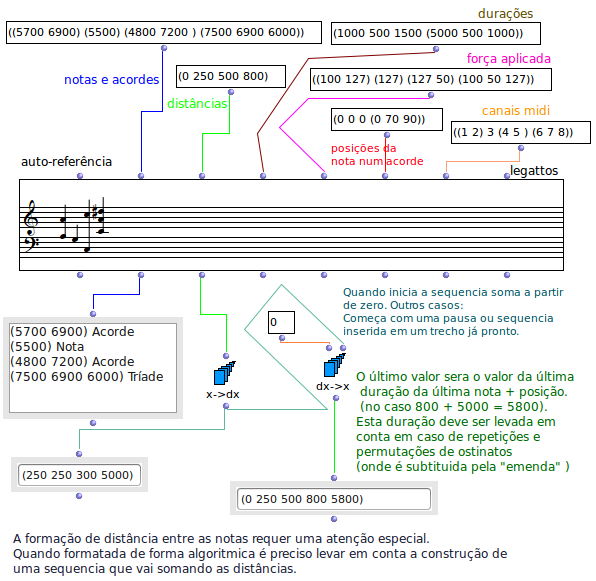
\includegraphics[scale=0.7]{OMPD/chord-seq-sem-titulo.png}
	\end{center}
	\legend{Fonte: autor }
\end{figure}



\subsubsection{Listas de dados}

O OM implementa uma série de operações sobre as listas de dados estruturadas. Abaixo selecionamos algumas funções básicas que auxiliam na manipulação dos dados dentro do OM.

\begin{figure}[!h]
	\caption{\label{fig_grafico}Operações com listas no OMs}
	\begin{center}
	    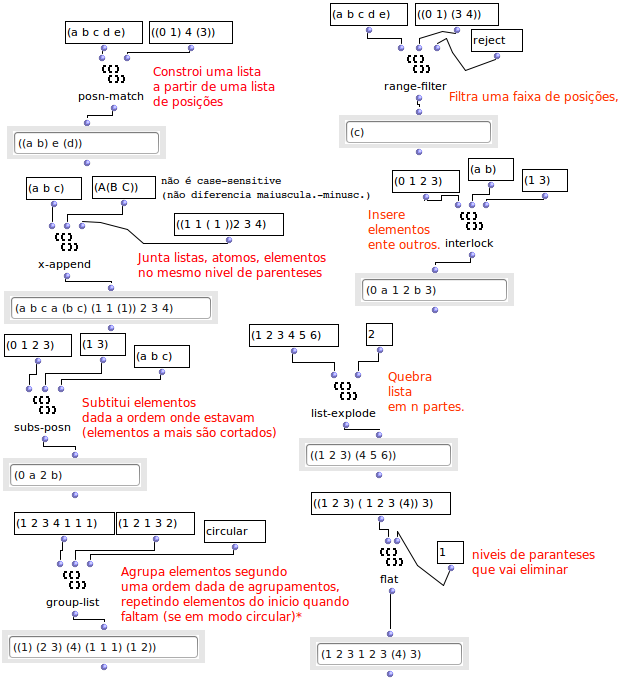
\includegraphics[scale=0.7]{OMPD/OM-listas01.png}
	\end{center}
	\legend{Fonte: autor }
\end{figure}

\begin{figure}[!h]
	\caption{\label{fig_grafico}Operações com listas no OMs}
	\begin{center}
	    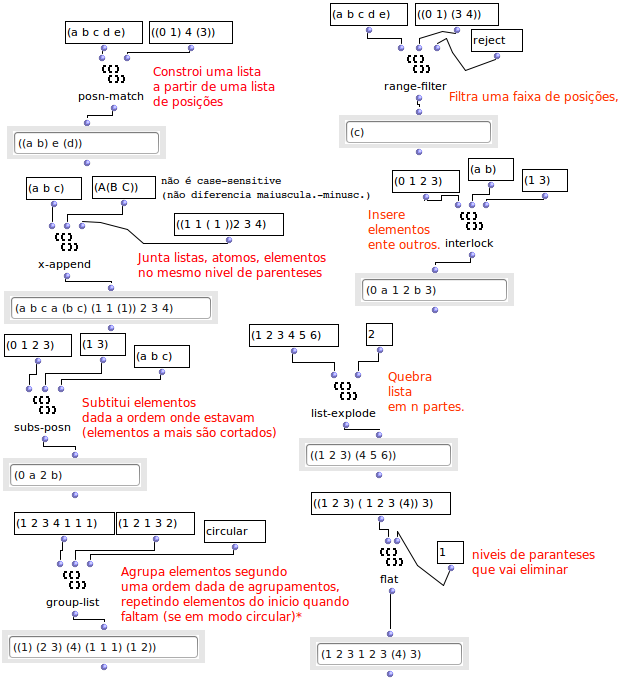
\includegraphics[scale=0.7]{OMPD/OM-listas01.png}
	\end{center}
	\legend{Fonte: autor }
\end{figure}


\subsubsection{Operações combinatórias e operações sobre grupos de classes de altura }
\label{OMmath}
O OM possui também algumas classes já preparadas especialmente para organizar séries, permutar, ordenar, embaralhar. Há inclusive uma classe chamada \textit{"math"}, que antecipa e organiza uma série de operações básicas sobre grupos de classes de altura, como extração do vetor intervalar, classificação de conjuntos de Allen Forte e uma representação gráfica da geometria das classes de altura, o objeto \textit{"n-cerle"} \cite{andreatta2003implementing}. Alguns objetos desta classe foram testados nas demonstrações do \autoref{modelos}.

\begin{figure}[!h]
	\caption{\label{fig_grafico}Alguns objetos para operações combinatórias e operações em grupos de classes de altura no OMs}
	\begin{center}
	    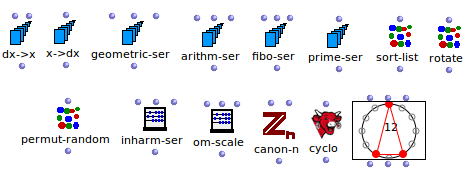
\includegraphics[scale=0.7]{OMPD/series-OM.png}
	\end{center}
	\legend{Fonte: autor }
\end{figure}

O OM também incorpora dentro de seus sequenciadores de nota um procedimento para segmentar articulações com fins de análise, preparando-os para uma classificação de grupos de alturas com a estrutura de dados do objeto \textit{"n-cercle"} \cite{bresson2012new}.

\begin{figure}[!h]
	\caption{\label{fig_grafico}Segmentação em Chord-Seq de OpenMusic}
	\begin{center}
	    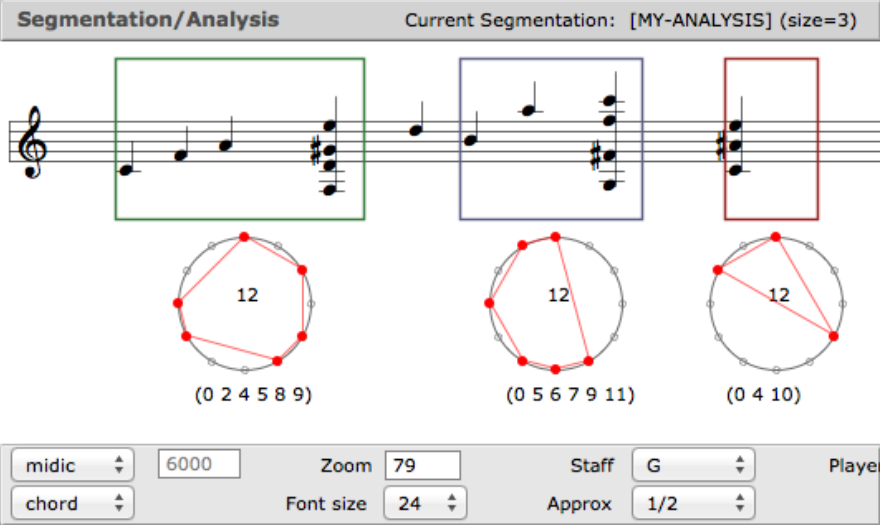
\includegraphics[scale=0.4]{OMPD/segmentaOM.png}
	\end{center}
	\legend{Fonte: \cite{bresson2012new} }
\end{figure}


\pagebreak
\subsection{PD}

Desde o início de seu desenvolvimento o PD surge como um software preocupado em resolver problemas de processamento digital de sinal de maneira estruturada - paralelo ao momento que sua versão comercial \textit{Max}\footnote{\url{http://cycling74.com/} Acesso em 10 de julho de 2014.} desenvolvia sua versão \textit{"MSP"}\ para processamento de áudio digital, baseada neste primeiro estágio do PD. 

\begin{citacao}
Um novo sistema de software, chamado \textit{Puredata}, está em seus primeiros estágios de desenvolvimento. Seu design almeja remediar algumas deficiências do programa Max e preservar algumas de suas vantagens. A mais importante fraqueza do Max é a dificuldade de manter estruturas de dados compostas de um tipo que possa ser acessado quando analisando e ressintetizando sons  ou quando gravando e modificando sequencias de diferentes tipos. Também, tem sido difícil integrar sinais que não sejam de áudio (vídeo por exemplo, e também espectro sonoro ) dentro do rígido sistema de “objetos til” ($\sim$ ) do Max. \cite{puckette1996pure}
\end{citacao}
 

Interessante perceber que já no final dos anos 90 o PD, tinha como alvo a vindoura possibilidade de uma música performática feita com os computadores domésticos que começavam a se popularizar, preocupando-se com aspectos de melhor performance de processamento de áudio, uso de video sincronizado e representação em tempo real de dados de processamento sonoro, apontando para a possibilidade de outros tipos de representação da música. Seu tutorial nativo é todo focado na didática do processamento digital de sinal. \cite{puckette2007theory}  

 
A música partiturada em \textit{scores} tradicionais nunca foi uma grande preocupação no PD. Podemos encontrar nativamente uma proposta de estrutura de dados mais próxima dos \textit{scores} eletroacústicos, como o de "Artikulation"\ de Ligeti ou "Studie II"\ de Stockhausen.\footnote{ c.f. "Solitude"\ de Hans C. Steiner:  \url{http://http://vimeo.com/16175509} Acesso em 10 de julho de 2014.}.


Apesar disso, vale lembrar também que, assim como o Max, o PD tem uma série de objetos preparados para lidar com o protocolo MIDI. Existem também várias bibliotecas de terceiros (distribuídas no pacote "Extended" ) que foram criadas pensando em manipulação de dados estruturados como semitons da escala de temperamento igual. Vejamos a seguir.

\begin{figure}[!h]
	\caption{\label{fig_grafico}Manipulação de arquivos MIDI no PD.}
	\begin{center}
	    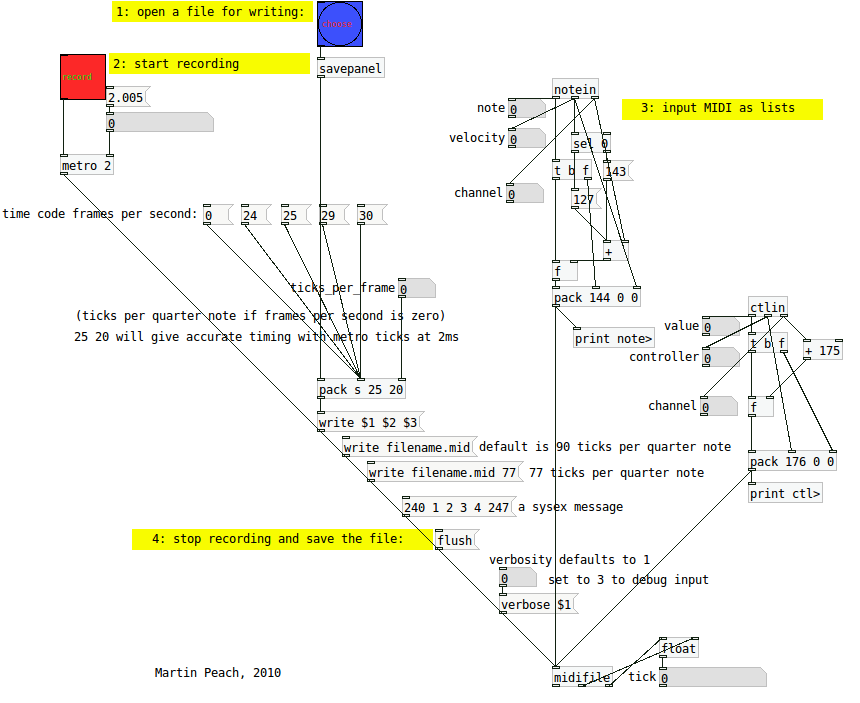
\includegraphics[scale=0.6]{OMPD/PD-midifile_write_-mrpeach.png}
	\end{center}
	\legend{Fonte: autor }
\end{figure}





\subsubsection{Biblioteca [RTC-lib]}


A biblioteca \textit{"Real Time Composition"} (RTC-lib) de Karheinz Essl, implementa algumas operações inspiradas em procedimentos seriais, algumas funções inclusive com nomes similares as do OM.

\begin{figure}[!h]
	\caption{\label{fig_grafico}Objetos da biblioteca "Real Time Composition"\ para PD.}
	\begin{center}
	    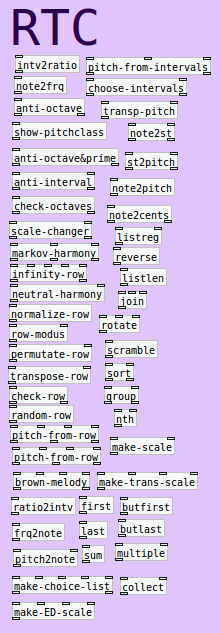
\includegraphics[scale=0.7]{OMPD/PD-RTC.png}
	\end{center}
	\legend{Fonte: autor }
\end{figure}

\subsubsection{Biblioteca de manipulação de listas [list-abs]}

Biblioteca que implementa diversas funções para busca, substituição, operações matemáticas, conversões de tipos, permutações e composições de listas de dados em forma de mensagens PD.

\begin{figure}[!h]
	\caption{\label{fig_grafico}Objetos da biblioteca "list-abs" para PD.}
	\begin{center}
	    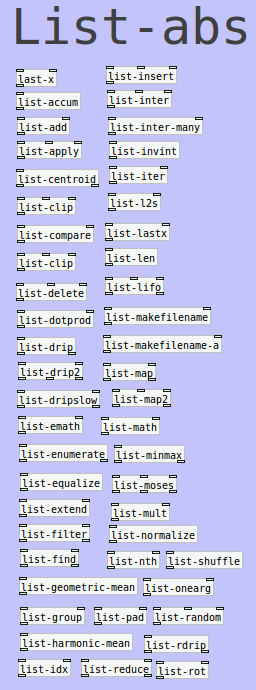
\includegraphics[scale=0.7]{OMPD/PD-list-abs.png}
	\end{center}
	\legend{Fonte: autor }
\end{figure}



\subsubsection{objeto [probalizer]}

Interessante implementação gráfica de histogramas que podem ser alimentados em tempo real, gerando números dentro da mesma probabilidade, encontrado na biblioteca \textit{"Unauthorized"}.

\begin{figure}[!h]
	\caption{\label{fig_grafico}Objeto [probalizer].}
	\begin{center}
	    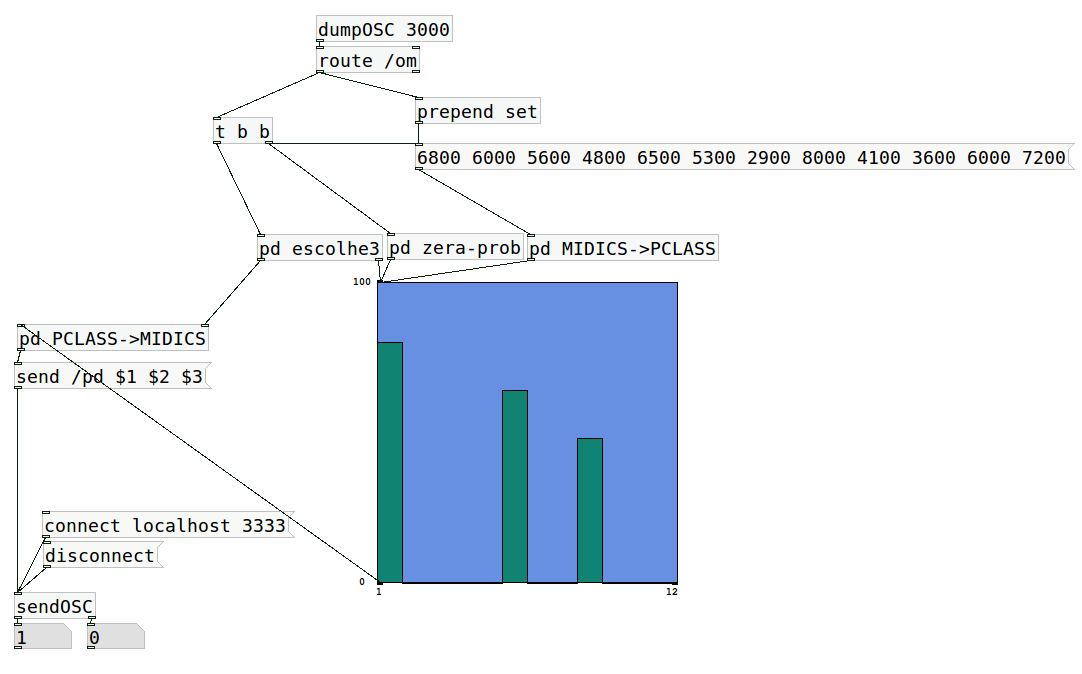
\includegraphics[scale=0.5]{OMPD/Probalizador-PD-OSC-OM.png}
	\end{center}
	\legend{Fonte: autor }
\end{figure}


% ----------------------------------------------------------
\chapter{Arquivos e Scripts para Segmentação de Dados Musicais}
% ----------------------------------------------------------
\label{formatos}

\section{MIDI}

Por muito tempo o formato MIDI ficou estigmatizado por ser associado aos timbres genéricos da indústria de sintetizadores populares dos anos 80 e 90 e pelas primeiras placas de som e softwares sequenciadores de eventos ou partituras dos computadores pessoais. 
Na verdade o formato não carrega parâmetros de timbres em seus metadados. Arquivo MIDI carrega valores básicos de expressão sobre a força que a nota de deve ser tocada e as alturas cromáticas que devem ser moduladas, permitindo que esta seja posteriormente associada a qualquer timbre.

A mensagem MIDI básica carrega informação sobre:

\begin{enumerate}

\item O canal onde vai atuar, permitindo mixar diversos instrumentos em polifonia.

\item O programa que indica o timbre.

\item \textit{NoteOn/NoteOff} - Nota soando e nota sem soar. O MIDI manda duas informações básicas sobre o envelope da nota. Uma primeira nota com a força inicial e uma segunda com a mesma nota e força zero, para silenciá-la.

\item \textit{Velocity} ou expressão: força com qual a nota é tocada.

\item Canal de controle para uso de escala de 127 passos que tem uso dependente da implementação da aplicação. Por exemplo, parâmetros de equalização do timbre. Na prática, o canal de controle é geralmente usado para receber dados de potenciômetros ou sensores analógicos e assinalar a qualquer tipo de parâmetro.

\item \textit{Pitch Bend} - Parâmetro para atuar diretamente na afinação de uma nota em tempo real, de modo similar ao gesto de \textit{bend} de instrumentos de cordas. A especificação MIDI permite que este controle tenha uma granulação de 16.384 pontos e geralmente é usada para um \textit{slide} que cobre duas oitavas.

\item Mensagens exclusivas de sistema (\textit{SysEx}) - geralmente usadas por aplicações para ações independentes do gesto musical. Por exemplo informar ao sistema onde onde buscar arquivos temporários de uma sessão.
\end{enumerate}

É importante ter em mente que o protocolo MIDI, por ser há mais de 35 anos um padrão ainda em uso, gerou um legado relevante de arquivos baseados em repertório clássico para a reconstituição de corpus de peças partituradas. Porém não são descritores capazes de garantir a boa formatação de seus dados como figuras de compasso de uma pauta tradicional, já que os arquivos MIDI não carregam informações sobre as figuras, apenas sobre suas durações, alturas e expressão. Quando importados para programas de notação ou convertidos para formatos destes, os arquivos MIDI irão passar por uma segmentação arbitrária e determinada pelo algoritmo \textit{"parser}"\footnote{Método computacional para conversão entre formatos ou tipos de dados diferentes.} que vai converter determinada duração em determinada métrica quantizada, normalmente diferente das articulações de quais as músicas foram digitalizadas.


Veremos a seguir outros arquivos mais específicos para este fim e quando necessário será feita a conversão entre os tipos.



\pagebreak

\section{Lilypond}

O objetivo principal no Lilypond é a formatação de uma notação partitural avançada e otimizada para impressão em papel. Permite também a utilização de elementos de notação mais exótica, inclusão de texto, dedilhados, nomenclatura de acordes, sinais de expressão, e customização de elementos a partir de módulos. Facilita a otimização da disposição e dimensão das fontes dos objetos e possui uma linguagem \textit{script} própria, dialeto da sintaxe \textit{scheme}\footnote{Tutorial oficial de lilypond-scheme: \url{http://lilypond.org/doc/v2.16/Documentation/source/Documentation/extending/introduction-to-scheme} Acesso em 10 de julho de 2014.}.



\begin{figure}[htb]
	\caption{\label{fig_grafico}Gerador de um acorde Dó maior (dó4 e4 g5) na clave de sol em Lilypond}
	\begin{center}
	    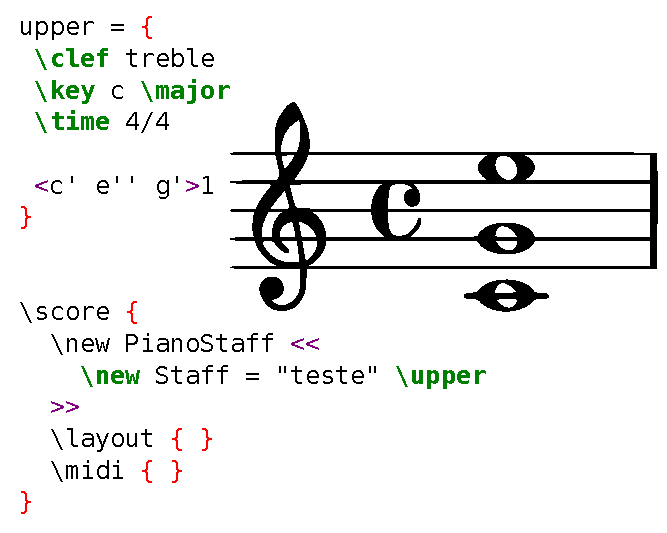
\includegraphics[scale=0.75]{score/lilypond.pdf}
	\end{center}
	%\legend{Fonte: autor}
\end{figure}




\section{MusicXML}

O uso geral do formato MusicXML é similar ao Lilypond - formatação de partituras. No entanto, enquanto Lilypond é um sistema completo fechado em si próprio, o MusicXML é um formato com a intenção de tornar-se um padrão intercambiável entre diferentes aplicações de partitura\footnote{ Lista atualizada de aplicações compatíveis com o formato MusicXML: \url{http://www.musicxml.com/software/} Acesso em 10 de julho de 2014.}.


\begin{figure}[htb]
	\caption{\label{fig_grafico}Gerador de uma nota dó4 na clave de sol em MusicXML}
	\begin{center}
	    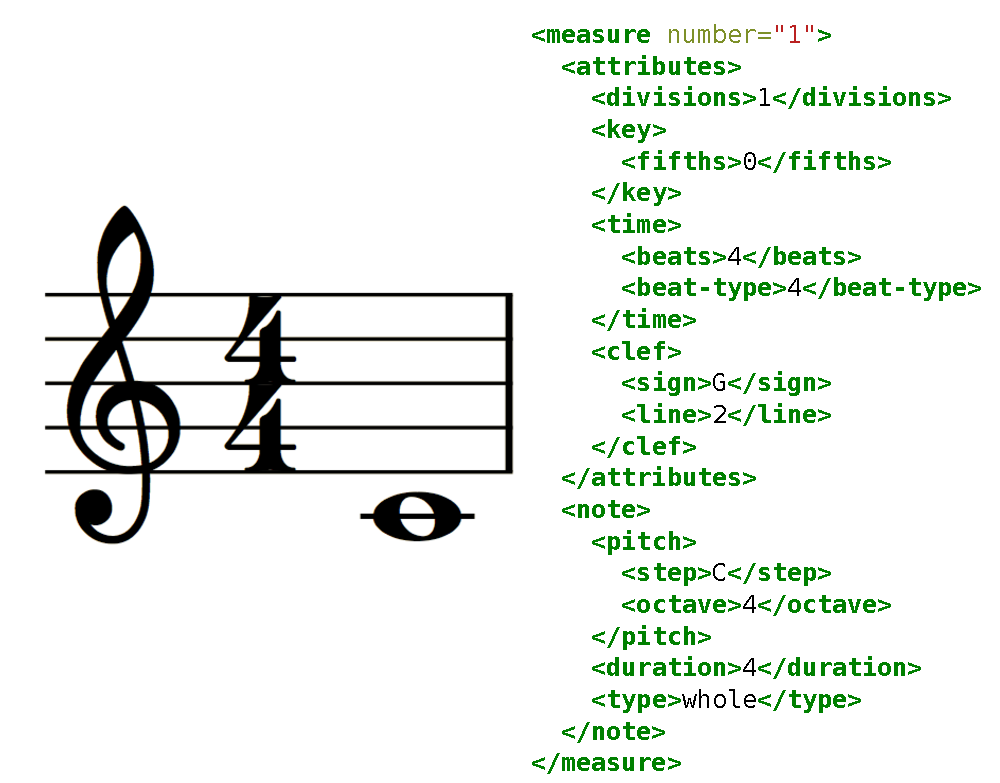
\includegraphics[scale=0.5]{score/musicxml.pdf}
	\end{center}
	%\legend{Fonte: autor}
\end{figure}

\pagebreak
\section{Bibliotecas Python auxiliares}

Pela sua natureza de código aberto alto-nível de orientação a objetos, Python \cite{van1995python} é uma linguagem \textit{script} que tem sido amplamente adotada e ampliada por bibliotecas para as mais diversas aplicações científicas e artísticas. \cite{downey2009python,Kroger201208}

Aliada ao uso de algumas bibliotecas específicas para arquivos de segmentação partitural, Python mostra-se uma ferramenta prática para formatação dinâmica de partituras prontas para impressão ou para auxiliar a análise de dados quantitativos de corpus de partituras.

Falaremos a seguir de duas dessas bibliotecas utilizadas como ferramenta auxiliar nesta pesquisa:


\subsection{Abjad}

É uma biblioteca voltada para a formatação de clichês em notação partitural pronta para impressão em papel, baseada na manipulação de \textit{templates} no formato Lilypond. A biblioteca apresenta alguns templates baseados em peças de Bártok, Ligeti, Ferneyhough e Mozart.\footnote{\url{http://abjad.mbrsi.org/examples/index.html} Acesso em 10 de julho de 2014.}



\subsection{Music 21}

É uma biblioteca projetada para trabalhar com manipulação e análise de \textit{corpus} de arquivos partituráveis\footnote{\url{http://web.mit.edu/music21/doc/moduleReference/moduleCorpus.html} Acesso em 10 de julho de 2014.}. Prepara a conversão entre diversos arquivos de dados musicais (MIDIs, humdrum, lilypond, abc)\footnote{\url{http://web.mit.edu/music21/doc/moduleReference/moduleConverter.html} Acesso em 10 de julho de 2014.}, mas nativamente trabalha com uma estrutura de dados baseada em Music XML.

Music21 tem uma abordagem voltada para uma "musicologia assistida por computador"\ e já tem incorporada em suas classes algumas ferramentas comuns a esta prática como: numeração de grau funcional de acorde\footnote{\url{http://web.mit.edu/music21/doc/moduleReference/moduleRoman.html} Acesso em 10 de julho de 2014.}, numeração de classes de altura usando a classificação de Allen Forte\footnote{\url{http://web.mit.edu/music21/doc/moduleReference/moduleChord.html?\#music21.chord.Chord.forteClassNumber} Acesso em 10 de julho de 2014.} e a implementação dos algoritmos de detecção de tonalidade\footnote{\url{http://web.mit.edu/music21/doc/moduleReference/moduleAnalysisDiscrete.html} Acesso em 10 de julho de 2014.} elaborado por \citeonline{krumhansl1990cognitive} e aperfeiçoado por \citeonline{temperley2001cognition}, descritos nesta pesquisa.\footnote{\autoref{perfiltonal}}









\part{Experimentos Composicionais Generativos}

\chapter{Gerador de MikroBagatellas}


\chapter{CosmoSonoridade de um Rascunho em Aberto }

Proponho aqui um experimento mais livre, 






% ---

% ---
% Conclusão (outro exemplo de capítulo s


% ---

% ---
% Conclusão (outro exemplo de capítulo sem numeração e presente no sumário)
% ---em numeração e presente no sumário)
% ---
\chapter*[Conclusão]{Conclusão}
\addcontentsline{toc}{chapter}{Conclusão}
\label{conclusao}
% ---

%\lipsum[31-33]

A busca por regras gerativas \cite{roads1979grammars} que pudessem formalizar algoritmos a partir de análises musicais de dados quantitativos capazes de segmentar e isolar parâmetros nos levou a encontrar uma interessante diferença entre duas abordagens analíticas que nos parecem complementares, apesar de contraditórias em certos aspectos.

Por um lado, revisamos uma corrente teórica que enumera estruturas operantes nas expectativas da música tonal. As argumentações derivadas da "Teoria Gerativa da Música Tonal" (GTTM) operam sobre aquele repertório considerado como prática comum nas análises funcionais das cadências, modulações, prolongamentos, tensão e relaxamento. Tais teorias argumentam que esta normatização é derivada de um condicionamento cultural na escuta da música ocidental e procuram justificar suas regras de "boa-formação" ou "preferência"\cite{lerdahl1983generative,temperley2001cognition} legitimando as fórmulas a partir de teses linguísticas das estruturas de sintaxe derivadas da fala e escrita \cite{chomsky1957syntactic} e as pesquisas de campo em cognição musical básica das relações entre intervalos e percepção subjetiva das alturas em seu espaço tonal inferido pelo ouvinte \cite{krumhansl1990cognitive,lerdahl2001tonal}. 

Por outro lado nos chamou atenção que em paralelo a fundamentação destas teorias, nas últimas décadas do século XX\footnote{A partir da sedimentação de uma tradição pós-tonal iniciada nas primeiras décadas do século XX.} formalizou-se uma "teoria de grupos das classes de altura"\cite{forte1973structure,rahn1980basic,perle1990pitch,straus2004} baseada numa catalogação de combinações de intervalos formando compostos sonoros singulares e as possíveis estruturações e articulações entre estes. Ali operariam critérios não necessariamente tão amarrados na funcionalidade dos esquemas de tensão e relaxamento das formas "tonalizantes". Mesmo que vertiginosamente, é preciso admitir que cada composição já pode comportar um sistema totalmente idiossincrático. Ao contrário da corrente cognitivista, neste caso uma criatividade autoral do analista assume que as formas estão emergindo ali a princípio porque foram apontadas, e não necessariamente porque foram intuídas pelo compositor. Também não buscam justificar expectativas do ouvinte que guiariam a normatização de uma busca composicional da "boa forma" pré-concebida \cite{babbitt1958cares}.

Dadas estas duas perspectivas pretendemos continuar este trabalho com uma organização dos algoritmos sugeridos por estas em bibliotecas das linguagens de programação apontadas na \autoref{computacional}, incluindo aí aprofundar e apontar boas práticas nas linguagens almejando uso otimizado destas teorias em processos composicionais. Nos interessa testar os limites práticos destas implementações, deixando um legado tecnicamente apropriável, utilizando ferramentas e bibliotecas auxiliares disponíveis em software livre.

Utilizaremos para exemplificar o uso das regras observadas em contextos tonais e pós-tonais alguns aspectos dos algoritmos atuando em um corpus de peças do repertório da suíte Mikrokosmos de Béla Bártok que será revisado no formato \textit{Music XML} para o estudo computacional, buscando respeitar a grafia das partituras originais. 

Partiremos de pistas já deixadas por autores que aprofundaram o tema \cite{marshall1946analysis,suchoff1971guide, lendvai1971bela,antokoletz1984music,suchoff2004bartok,lester1989analytic}.

Mais do que encontrar alguma nova abordagem analítica sobre estas peças, buscaremos a demonstração de algumas regras gerativas observadas, para em seguida serem utilizados de maneira mais livre em procedimentos composicionais que gerem motivos partiturados - e sugestões de encadeamento destes.

Composições produzidas durante esta pesquisa estão disponíveis para \textit{download}\footnote{\url{http://http://vimeo.com/16175509} Acesso em 10 de julho de 2014.}. Também estão disponíveis os códigos que estão sendo trabalhados\footnote{\url{https://github.com/glerm/luteriaOM}, \url{https://github.com/glerm/Derivas_OpenMusic} e \url{https://github.com/glerm/AutomatosGeradores} Acesso em 10 de julho de 2014. }. A próxima etapa será modularizar e comentar os códigos, detalhando os processos da maneira mais didática possível.

Vale lembrar que estamos convencidos de que uma abordagem analítica que desconsidere parâmetros determinantes sobre a sonoridade \cite{guigue2012} dos aglomerados de alturas, como parte intencional e determinante na composição estará incompleta. Também acreditamos que é limitador ignorar a tipo-morfologia \cite{shaeffer1966traite} e espectro-morfologia \cite{smalley1997spectromorphology} dos timbres atuantes numa situação real de gravação, performance partiturada ou improviso sobre as estruturas geradas. Interessa-nos refletir sobre estes aspectos em alguma continuidade deste trabalho.




% ----------------------------------------------------------
% ELEMENTOS PÓS-TEXTUAIS
% ----------------------------------------------------------
\postextual
% ----------------------------------------------------------

% ----------------------------------------------------------
% Referências bibliográficas
% ----------------------------------------------------------
%\bibliography{abntex2-modelo-references}
\bibliography{mestrado_glerm}
% ----------------------------------------------------------
% Glossário
% ----------------------------------------------------------
%
% Consulte o manual da classe abntex2 para orientações sobre o glossário.
%
%\glossary

% ----------------------------------------------------------
% Apêndices
% ----------------------------------------------------------

% ---
% Inicia os apêndices
% ---
%\begin{apendicesenv}

% Imprime uma página indicando o início dos apêndices
%\partapendices




%%%%

%\chapter{Repositório de Códigos}
%\label{codigo}


%\subsection{Biblioteca de Algoritmos}



%\lstset{frameround=fttt,language=Python,showspaces=false,
%showtabs=true,tab=\rightarrowfill}
%\begin{lstlisting}[frame=trBL]
%def mod12(n):
%	return n % 12
%
%def note_name(number):
%	notes = "C  D E F G A B".split()
%	return notes[mod12(number)]
%	
%for i in intervalos:
%	if (i in maiores):
%		if (i == (4,7)):
%			tipos.append(("maior",0))
%		if (i == (5,9)):
%			tipos.append(("maior",1))
%		if (i == (3,8)):
%			tipos.append(("maior",2))
% 
%	if (i in menores):
%		if (i == (3,7)):
%			tipos.append(("menor",0))
%		if (i == (5,8)):
%			tipos.append(("menor",1))
%		if (i == (4,9)):
%			tipos.append(("menor",2))
%	if (i in aumentados):
%			tipos.append(("aumentado","not"))
%	if (i in diminutos):
%		if (i == (3,6)):
%			tipos.append(("diminuto",0))
%		if (i == (6,9)):
%			tipos.append(("diminuto",1))
%		if (i == (3,9)):
%			tipos.append(("diminuto",2))
% 
%\end{lstlisting}





%\end{apendicesenv}
% ---


% ----------------------------------------------------------
% Anexos
% ----------------------------------------------------------

% ---
% Inicia os anexos
% ---
%\begin{anexosenv}

% Imprime uma página indicando o início dos anexos
%\partanexos



% ---
%\chapter{Regras da Teoria Gerativa da Musica Tonal}
% ---


%\end{anexosenv}

%---------------------------------------------------------------------
% INDICE REMISSIVO
%---------------------------------------------------------------------
\phantompart
\printindex
%---------------------------------------------------------------------

\end{document}
